
% part 15
\section{Протестированная поэзия\label{sec:part15}}

\subsection{Введение}

Мы написали много кода для того, чтобы изучить Twisted, но 
до сих пор мы пренебрегали написанием тестов. 
Вы можете удивиться: ``Как можно тестировать асинхронный код 
используя синхронную систему, подобную пакету 
\href{http://docs.python.org/library/unittest.html#module-unittest}{unittest} 
из Python'а?'' Короткий ответ: вы не можете. Как мы обнаружили, 
синхронный и асинхронный код не смешиваем, по меньшей мере не без труда.


К счастью, Twisted включает свою собственную 
тестирующую систему, названную 
\href{http://twistedmatrix.com/documents/current/core/howto/testing.html}{trial}, 
которая поддерживает тестирование асинхронного кода (также ее можно 
использовать для тестирования сихронного кода).


Мы будем предполагать, что вы уже знакомы с 
основными механизмами unittest и подобными 
тестирущими системами, в которых вы создаете 
тесты определением класса с определенным родительским 
классом (обычно с названием TestCase), 
и каждый метод того класса, начинающийся со слова ``test'', 
считается одним тестом. Система заботится об обнаружении 
всех тестов, запускаемых один за другим с опциональными 
шагами setUp и tearDown, а также сообщает о результатах. 


\subsection{Пример}

%You will find some example tests located in tests/test\_poetry.py. To ensure all our examples are self-contained (so you don’t need to worry about PYTHONPATH settings), we have copied all the necessary code into the test module. Normally, of course, you would just import the modules you wanted to test.

Вы найдете некоторые примеры тестов в 
\href{http://github.com/jdavisp3/twisted-intro/blob/master/tests/test\_poetry.py#L1}{tests/test\_poetry.py} . Для гарантии автономности (то есть 
не надо беспокоиться о настройках PYTHONPATH) мы скопировали 
весь необходимый код в модуль test. Обычно, конечно же, вы могли бы 
просто импортировать модули, которые вы бы хотели проверить.


Слудующий тест проверяет поэтический клиент и сервер, используя клиент 
для поэмы из тестового сервера. Для того, чтобы запустить 
сервер для тестирования, мы реализовали метод 
\href{http://github.com/jdavisp3/twisted-intro/blob/master/tests/test\_poetry.py#L70}{setUp} 
в качестве нашего testcase'а:

\begin{scriptsize}\begin{verbatim}
class PoetryTestCase(TestCase):

    def setUp(self):
        factory = PoetryServerFactory(TEST_POEM)
        from twisted.internet import reactor
        self.port = reactor.listenTCP(0, factory, interface="127.0.0.1")
        self.portnum = self.port.getHost().port
\end{verbatim}\end{scriptsize}


%The setUp method makes a poetry server with a test poem, and listens on a random, open port. We save the port number so the actual tests can use it, if they need to. And, of course, we clean up the test server in tearDown when the test is done:

Метод setUp создает сервер с тестовой поэмой и слушает случайный, 
открытый порт. Мы сохраняем номер порта, поэтому тесты могут его 
использовать. И, конечно же, мы завершаем тестовый сервер в 
функции 
\href{http://github.com/jdavisp3/twisted-intro/blob/master/tests/test\_poetry.py#L76}{tearDown}, 
когда тесты завершены:

\begin{scriptsize}\begin{verbatim}
    def tearDown(self):
        port, self.port = self.port, None
        return port.stopListening()
\end{verbatim}\end{scriptsize}

В нашем первом тесте 
\href{http://github.com/jdavisp3/twisted-intro/blob/master/tests/test\_poetry.py#L80}{test\_client} 
мы используем get\_poetry для того, чтобы получить поэму 
из тестового сервера, и проверяем, что это та самая поэма, которую мы ожидаем:

\begin{scriptsize}\begin{verbatim}
    def test_client(self):
        """The correct poem is returned by get_poetry."""
        d = get_poetry('127.0.0.1', self.portnum)

        def got_poem(poem):
            self.assertEquals(poem, TEST_POEM)

        d.addCallback(got_poem)

        return d

\end{verbatim}\end{scriptsize}


Заметим, что наша тестовая функция возвращает deferred. 
При использовании trial, каждый метод выполняется как 
callback. Это означает, что reactor выполняется и  мы 
можем производить асинхронные операции как часть теста. 
Нам только нужно дать системе знать, что наш тест асинхронный, 
и мы делаем это обычным способом - возвращаем deferred.


Система trial будет ждать до тех пор пока deferred не 
активизируется вызовом метода tearDown, и завершит тест 
с ошибкой, если deferred не выполнится (например, если 
последяя пара callback/errback завершилась с ошибкой). 
Наш тест также провалится, если наш deferred слишком 
долго активизируется (по умолчанию - 2 минуты). Это означает, 
что если тест завершился, мы знаем, что наш deferred 
активизировался, и поэтому наш callback 
активизировался и запускал метод assertEquals.


Наш второй тест, 
\href{http://github.com/jdavisp3/twisted-intro/blob/master/tests/test\_poetry.py#L91}{test\_failure}, 
проверяет, что get\_poetry завершается с ошибкой 
определенным образом, если мы не можем соединиться 
с сервером:

\begin{scriptsize}\begin{verbatim}
    def test_failure(self):
        """The correct failure is returned by get_poetry when
        connecting to a port with no server."""
        d = get_poetry('127.0.0.1', -1)
        return self.assertFailure(d, ConnectionRefusedError)

\end{verbatim}\end{scriptsize}


Здесь мы пытаемся подсоединиться к невалидному 
порту и затем используем метод assertFailure из trial'а. Этот 
метод подобен иметоду assertRaises из модуля unittest, но 
используется для тестирования асинхронного кода. Он 
возвращает deferred, который успешно завершается, если 
заданный deferred генерирует заданное исключение, 
иначе - завершается с ошибкой.


вы можете самостоятельно запускать тесты, используя скрипт trial 
следующим образом:

\begin{scriptsize}\begin{verbatim}
trial tests/test_poetry.py
\end{verbatim}\end{scriptsize}


И вы увидете некоторый вывод, показывающий 
каждый testcase и OK, сообщающий, что каждый 
тест пройден успешно.


\subsection{Обсуждение}

Поскольку trial похож на unittest в отношении 
к основному API, то достаточно просто начать писать тесты. 
Нужно только возвратить deferred, если Ваш тест использует 
асинхронный код, и trial позаботится обо всем. вы также можете 
возвращать deferred из методов setUp и tearDown, если 
они должны быть также асинхронными. 


Любые логи из Ваших тестов будут собираться в файле 
внутри директории с названием \_trial\_temp, 
которую trial создаст автоматически, если ее нет. 
В дополнение к ошибкам, напечатанным на экране, 
лог - полезная начальная точка при отладке тестов с ошибками. 

Рисунок \ref{fig:test-1} показывает гипотетический тест в 
процессе запуска:

\begin{figure}[h]
\begin{center}
    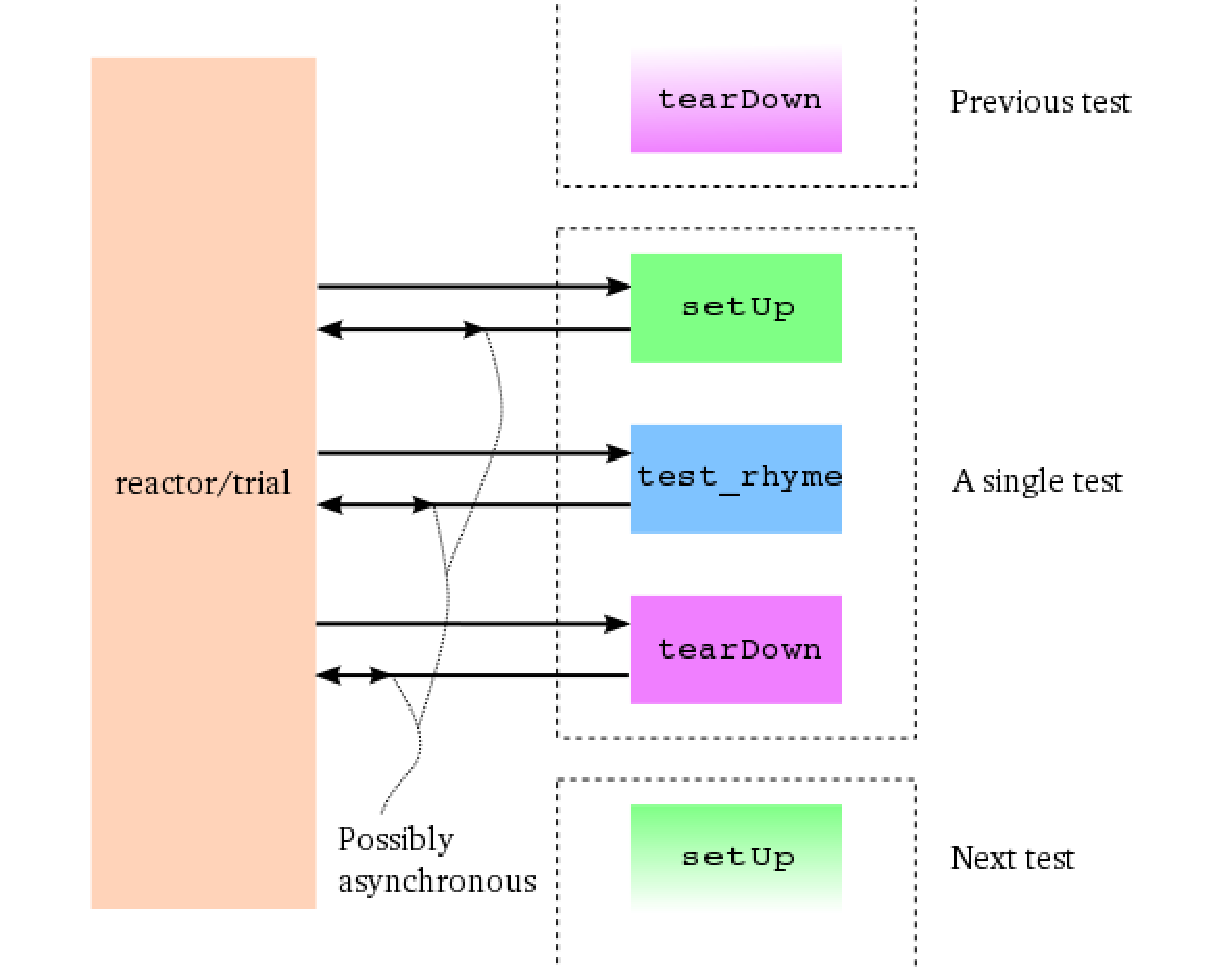
\includegraphics[width=0.8\textwidth]{images/test-1.pdf}
    \caption{Запущенный trial тест\label{fig:test-1}}
\end{center}
\end{figure}


Если вы когда-нибудь использовали подобные системы ранее, 
то вы должны быть знакомы с моделью, за исключением того, что 
все относящиеся к тестам методы могут возвращать deferred'ы.

Система trial - хорошая иллюстрация того как 
``работающая асинхронность'' вызывает изменения во всей программе. 
Для того, чтобы тест (или любая функция) был асинхронным, он должен:

\begin{enumerate}

\item Не блокироваться
\item Зачастую, возвращать deferred

\end{enumerate}


Но это означает, что любые вызовы функции должны 
готовы принять deferred и не блокироваться (
возможно, также возвращать deferred). И так это условие 
распостраняется далее. Таким образом, возникает необходимость в системе, 
подобной trial, которая может управлять асинхронными тестами, которые 
возвращают deferred'ы.

\subsection{Резюме}

Если вы хотите посмотреть больше 
примеров о том как писать unit тесты для кода Twisted, 
вам нужно смотреть не дальше, чем сам Twisted. Twisted 
имеет очень много unit тестов, с новыми добавленными при  
выходе каждого релиза. Поскольку эти тесты изучены 
Twisted экспертами, они являются прекрасным примером того, как 
правильно тестировать Twisted код.


В главе 16 мы будем использовать Twisted для того, чтобы 
сделать наш поэтический сервер подлинным демоном.

\subsection{Упражнения}

\begin{enumerate}

\item Поменяйте один из тестов так, чтобы вызвать ошибку, и 
запустите trial снова, чтобы посмотреть вывод программы.

\item Почитайте \href{http://twistedmatrix.com/documents/current/core/howto/testing.html}{документацию по тестирования в Twisted}\footnote[1]{http://twistedmatrix.com/documents/current/core/howto/testing.html}.

\item Напишите тесты для других поэтических сервисов.

\item Исследуйте \href{http://twistedmatrix.com/trac/browser/trunk/twisted/test}{некоторые тесты} в 
Twisted\footnote{http://twistedmatrix.com/trac/browser/trunk/twisted/test}.

\end{enumerate}

